\section{Evaluation}

\subsection{RTT Estimation}
We first define the RTT in RLC layer. In the RLC protocol, the STATUS PDUs (ACK or NACK) don't generate by every received RLC PDU, but triggered either by receiving a polling request from the sender or by detecting one or more missed PDUs from its receiver buffer~\cite{spec-3G-RLC}. Since the QxDM traces are collected at the client side, we don't have the information of when the server side receive the PDU. Thus, I estimate the RTT of a RLC PDU based on the timestamp difference between the most recent sender's polling request and received ACK. Based on RLC configuration, the maximum polling request frequency is 500 ms. One of the previous mobile RTT estimation study shows the autocorrelation coefficient of two RTT measurements within 500 ms is more than 0.6~\cite{proteus}. Therefore, my estimation is still reasonable to be considered as the real RLC RTT value.

\subsection{Cost-Benefit Analysis}
In order to know whether the new proposed RLC mechanism works, I apply a cost-benefit analysis over the existing \emph{TCP\_{}Trace}. The definition of benefit and cost is straight forward. Basically, if the fast retransmitted PDUs will be transmitted in the future, then we compare the RTT if it transmitted right after the duplicate ACKs with the real RTT value in the trace. If the difference is less than 0, we call that is a benefit. In the same way, if it is greater than 0, we call it a cost. However, we want to know if the PDU is really lost over the channel, or it just gets delayed due to channel contention. That depends on whether the sender receives a ACK or NACK (a list of unreceived PDU sequence numbers). We categorize the situations into four cases -- Win, Draw\_{}Plus, Draw\_{}Minus, and Loss. If the sender will receive a NACK, and more than 50\% of the fast retransmitted PDUs will retransmit in the real trace, then we call the case "Draw\_{}Plus" as in Figure~\ref{fig:draw.plus}. Since it would brings us benefit if the fast retransmit RTT is less than the RTT in the real trace. The "Win" case is defined that if we could avoid a TCP RTO based on the "Draw\_{}Plus" in Figure~\ref{fig:win}. In that case, RLC layer benefit is the same as "Draw\_{}Plus", but I want to highlight that it could bring further latency benefit over the transport layer. "Draw\_{}Minus" occurs when less than 50\% of the fast retransmitted PDUs get really retransmitted in the real trace as in Figure~\ref{fig:draw.minus}. If the sender gets a ACK with a larger sequence number, then all the PDUs were successfully delivered to the receiver. In that case, we called the case "Loss", since all the retransmitted packets are redundant as in Figure~\ref{fig:loss}. 

As we can see from Table~\ref{tab:rlc.fast.sim}, around 75\% of the time we will have benefit on RLC latency reduction if we count the "Win" and "Draw\_{}Plus". The overall RLC delay could be reduced by \textit{2.66\%} over all the RRC state based on trace simulation analysis. If we break down the cost-benefit over different RRC states, the RLC RTT latency could reduce by up to \textit{35.69\%} over initial FACH state or FACH promotion transitions. Therefore, we could have a large latency benefit over the initial period of data transmission.


% Four cases
\begin{figure}
\centering
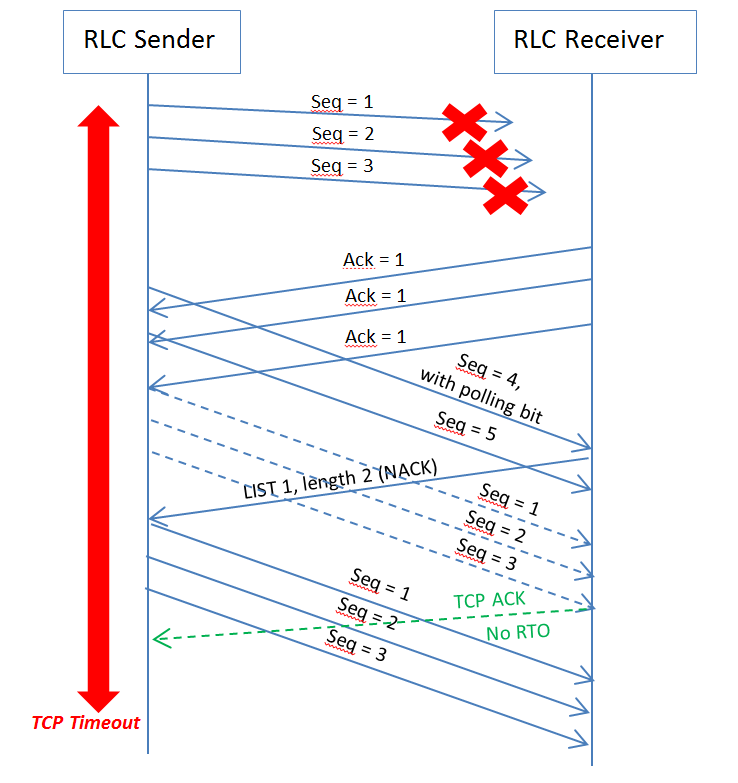
\includegraphics[width=0.45\textwidth]{figs/Win.png}
\caption{Win: RLC Fast Re-Tx avoid a TCP RTO}
\label{fig:win}
\end{figure}

\begin{figure}
\centering
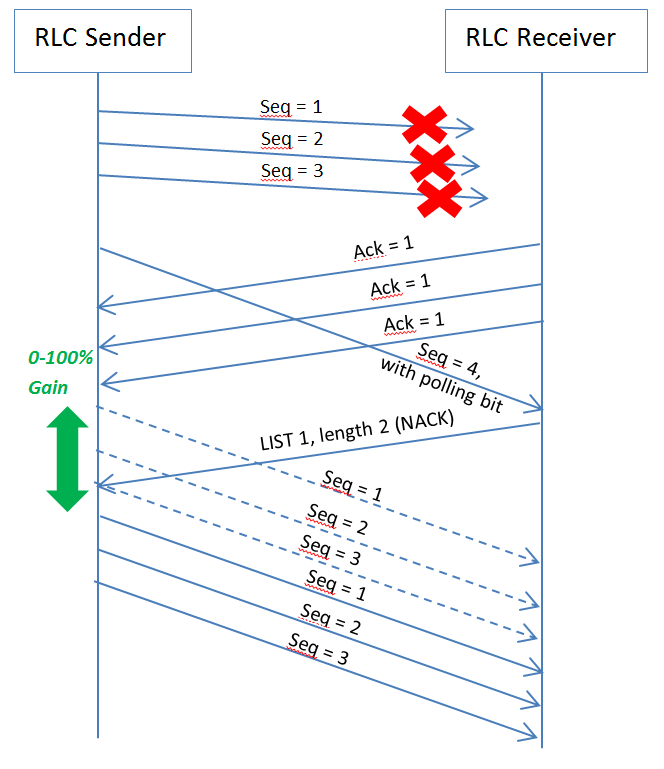
\includegraphics[width=0.45\textwidth]{figs/Draw_plus.png}
\caption{Draw Plus: the predication accuracy is more than 50\%}
\label{fig:draw.plus}
\end{figure}

\begin{figure}
\centering
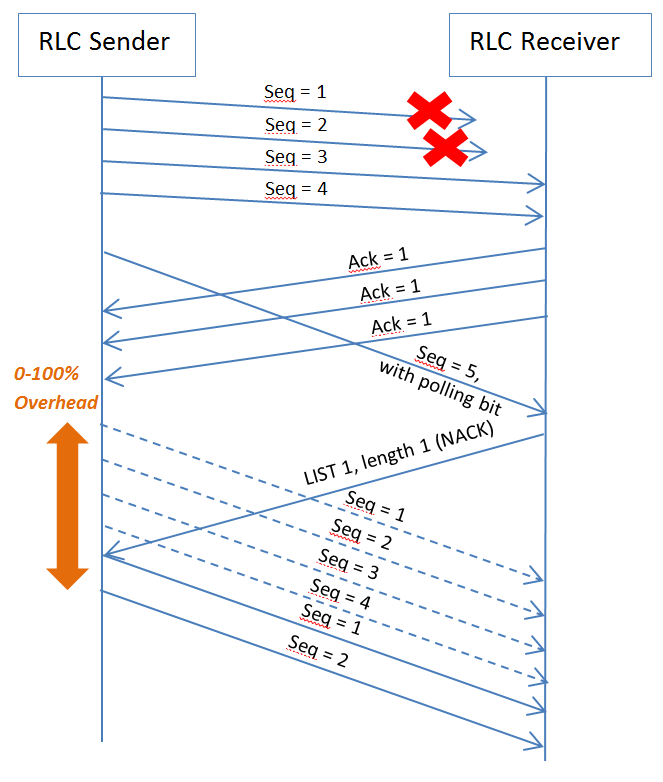
\includegraphics[width=0.45\textwidth]{figs/Draw.png}
\caption{Draw Minus: the predication accuracy is less than 50\%}
\label{fig:draw.minus}
\end{figure}

\begin{figure}
\centering
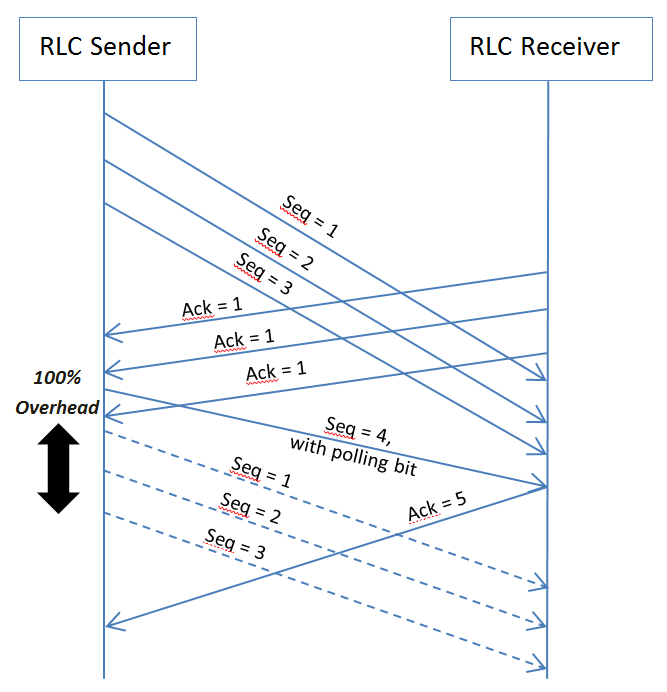
\includegraphics[width=0.45\textwidth]{figs/Loss.png}
\caption{Loss: all predications fail}
\label{fig:loss}
\end{figure}

% Cost-Benefit Table
\begin{table}
\begin{tabularx}{0.48\textwidth}{ | c | X |}
	\hline
	\textbf{Case Name} & \textbf{Percentage of Occurrence (\%)} \\
	\hline\hline
  	Win & 10.32$\pm$1.89 \\
  	\hline
  	Draw\_{Plus}* & 64.68$\pm$8.32 \\
  	\hline
  	Draw\_{Minus} & 20.63$\pm$3.45 \\
  	\hline
  	Loss & 4.25$\pm$0.06 \\
  	\hline
\end{tabularx}
* The Draw\_{Plus} case excludes the percentage of Win
\caption{The RLC Fast Re-Tx Cost-Benefit Table}
\label{tab:rlc.fast.sim}
\end{table}


\label{sec:eval}

